\documentclass[a4paper,11pt,fleqn]{report}
\usepackage[utf8]{inputenc}
\usepackage{graphicx}
\usepackage{listings}
\usepackage{rotating}
\usepackage[hidelinks]{hyperref}
\usepackage[space]{grffile}
\usepackage{amsmath}
\usepackage{array}
\usepackage{longtable}
\everymath{\displaystyle}

% Title Page
\title{\textbf{Test Plan Document}}
\author{
  Michele Madaschi
  \and
  Lidia Moioli
  \and
  Luca Martinazzi  % last but not least
}

\begin{document}
\maketitle
\tableofcontents

\chapter*{Introduction}
\addcontentsline{toc}{chapter}{Introduction}
\setcounter{section}{0}
\addtocounter{chapter}{1}

\section{Revision History}
First version (1.0) of the ITPD document.
\section{Purpose and Scope}
This document aims to describe, specify and analyze the integration test strategy for \textit{My Taxi Service}, 
in terms of the components/classes to integrate and the typology of testing, while also providing a 
general schedule for the whole process; all is done accordingly to what was established in the previous assignments. \\


\section{List of Definitions and Abbreviations}
\begin{itemize}
 \item RASD: Requirements Analysis and System Design
 \item DD: Design Document
\item ITPD: Integration Test Plan Document
\end{itemize}

\section{List of Reference Documents}
\begin{itemize}
\item The project description.
\item Our RASD document.
\item Ou DD document.
\end{itemize}
 
%Internal Logic File: users(x3), ride, sharedride, taxiqueue (il set di coordinate è incluso nelle taxiqueue)
%External Interface File: gps coordinates, map service
%External Input: login,logout, request, reserve,delete, reserve shared, accept call, refuse call  report, master terminal functions
%External Output:message (eta, no taxi message)
%External Inquiry: see profile, see active ride list
\chapter*{Function Points} 
\addcontentsline{toc}{chapter}{Function Points}
\setcounter{section}{0}
\addtocounter{chapter}{1}
In order to evaluate the cost of the project we have to identify 
the function points and estimate the complexity of each one.
To each point we assign a weight referring to this table:\\

\begin{tabular}{ | c | l | l | l |}
    \hline
     Function types & \multicolumn{3}{|c|}{Weight} \\\hline
       & Simple  & Medium & Complex \\ \hline
    External Input & 3 & 4 & 6   \\ \hline
    External Output & 4 & 5 & 7 \\ \hline
    External Inquiry & 3 & 4  & 6 \\ \hline
    Internal Logic File & 7 & 10 & 15 \\ \hline
    External Interface File & 5 & 7 & 10  \\ \hline
    \end{tabular}

\begin{itemize}
  \item{\makebox{Internal Logic File\hfill}: users (guest, taxidriver and passenger), 
                               ride, sharedride, taxiqueue}
  \item{\makebox{External Interface File\hfill}: gps coordinates, map service}
  \item{\makebox{External Input\hfill}: login, logout, request, reserve, delete, reserve shared,
                         accept call, refuse call, report, taxi available,
                         taxi not available, change settings}
  \item{\makebox{External Output\hfill}: message (eta, no taxi message)}
  \item{\makebox{External Inquiry\hfill}: see profile, see active ride list}
\end{itemize}


\section{Complexity and cost evaluation}
  \subsection{Internal Logic File}
  According to our previous specification (explained in the RASD and DD documents),
  users and ride have to store few informations, thus we can adopt the
  simple cost weight for those ones.
  On the other hand, \textbf{sharedride} and \textbf{taxiqueue} have to store a dynamic
  list, that require more attention, so we adopt a medium cost weight.
  \begin{equation}
   4*7 + 2*10 = 48 \text{ FPs}
  \end{equation}

  \subsection{External Interface File}
  The interactions with \textbf{gps} coordinates and the \textbf{map service} are very simple, 
  because we need to gather few information from them, so we adopt a simple weight for
  both of External Internal Files.
  \begin{equation}
   2*5 = 10 \text{ FPs}
  \end{equation}
  
  \subsection{External Input}
  Most of the external inputs are simple actions involving a few number of entities,
  therefore we can adopt a simple weight cost for all of them.
  \textbf{request} and \textbf{change settings} however are more complex, and thus require a medium weight cost.
  \begin{equation}
    10*3 + 2*4= 38 \text{ FPs}
  \end{equation}
  
  \subsection{External Output}
  Sending \textbf{eta} requires to access the map service that calculate, on its own,
  the appropriate value, so we adopt a simple cost weight for message.
  \begin{equation}
    2*4 = 8 \text{ FPs}
  \end{equation}
  
  \subsection{External Inquiry}
  \textbf{see profile} requires only to send some fields saved in the current user,
  while \textbf{see active ride} list requires to scan the ridehistory and check its status (active or not).
  Therefore, we adopt a simple cost weight for the former, and a medium cost weight for the latter.
  \begin{equation}
    1*3 + 1*4 = 7 \text{ FPs}
  \end{equation}
  
  \subsection{Overall}
  In summary we have $\text{FPs} = \sum_{i=1}^{5} \text{FP}i = 111 $
 

%effort=2.94*EAF*(KLOC)^E
%duration=3.67*(effort)^Se
%Npeople=effort/duration
\chapter*{COCOMO II}
\addcontentsline{toc}{chapter}{COCOMO II}
\setcounter{section}{0}
\addtocounter{chapter}{1}
%\section{Integration test case I-1}
\begin{tabular*}{1.23\textwidth}{ l l }
 \textbf{Test Case Identifier}		& I-1-T1 \\
 \hline
 \textbf{Test Item(s)}			& Ridesmanager $\rightarrow$ Controller \\
 \hline
 \textbf{Input specification}		& Create the typical Ridesmanager input \\
 \hline
 \textbf{Output specification}		& Check if the correct methods are called in the Controller \\
 \hline
 \textbf{Environmental needs}		& Ridesmanager driver \\
\end{tabular*}

\section{Integration test case I-2}
\begin{tabular*}{1.23\textwidth}{ l l }
 \textbf{Test Case Identifier}		& I-2-T1 \\
 \hline
 \textbf{Test Item(s)}			& Controller $\rightarrow$ GuestController \\
 \hline
 \textbf{Input specification}		& Create the typical Controller input \\
 \hline
 \textbf{Output specification}		& Check if the correct methods are called in the GuestController \\
 \hline
 \textbf{Environmental needs}		& I-1 succeeded \\
\end{tabular*}

\section{Integration test case I-3}
\begin{tabular*}{1.23\textwidth}{ l l }
 \textbf{Test Case Identifier}		& I-3-T1 \\
 \hline
 \textbf{Test Item(s)}			& Action $\rightarrow$ LoginAction \\
 \hline
 \textbf{Input specification}		& ?? \\
 \hline
 \textbf{Output specification}		& ?? \\
 \hline
 \textbf{Environmental needs}		& ?? \\
\end{tabular*}

% [...] things to clarify たすけてくれて、Luca-くん

\section{Integration test case I-X4}
\begin{tabular*}{1.23\textwidth}{ l l }
 \textbf{Test Case Identifier}		& I-X4-T1 \\
 \hline
 \textbf{Test Item(s)}			& ClientNetworkInterface $\rightarrow$ ClientMessage \\
 \hline
 \textbf{Input specification}		& Invoke various types of network methods \\
 \hline
 \textbf{Output specification}		& Check that the correct ClientMessage(s) are generated \\
 \hline
 \textbf{Environmental needs}		& ClientNetworkInterface driver \\
\end{tabular*}

\section{Integration test case I-X5}
\begin{tabular*}{1.23\textwidth}{ l l }
 \textbf{Test Case Identifier}		& I-X5-T1 \\
 \hline
 \textbf{Test Item(s)}			& ServerNetworkInterface $\rightarrow$ ServerMessage \\
 \hline
 \textbf{Input specification}		& Invoke various types of network methods \\
 \hline
 \textbf{Output specification}		& Check that the correct ServerMessage(s) are generated \\
 \hline
 \textbf{Environmental needs}		& ServerNetworkInterface driver \\
\end{tabular*}



 \chapter*{Schedule and resources allocation}
 \addcontentsline{toc}{chapter}{Schedule and resources allocation}
 \setcounter{section}{0}
 \addtocounter{chapter}{1}
 \section{ Gantt's diagram}
For this project we had to arrange several deliverables, each one with a strict deadline.
In particular:
\begin{enumerate}
\item RASD - 06/11/2015
\item DD - 04/12/2015
\item INSPECTION - 05/01/2016
\item INTEGRATION TESTING - 21/01/2016
\item PROJECT PLANNING - 02/02/2016
\end{enumerate}

To accomplish the work we folllowed the instructions of each assignment, referring 
to course material and past years projects.\\
Our team strategy was definying  all together the main guidelines of the document to be created, with one 
scribe. Then at home each of us expanded and clarified the content previously decided.\\
A special case was the inspection document, when we associated randomly the points in the checklist to each member.\\
The whole project lasted 4 months, with an individual work of 110 hours/person approximately.

\begin{center}
\begin{figure} [h]

\noindent\makebox[\textwidth]{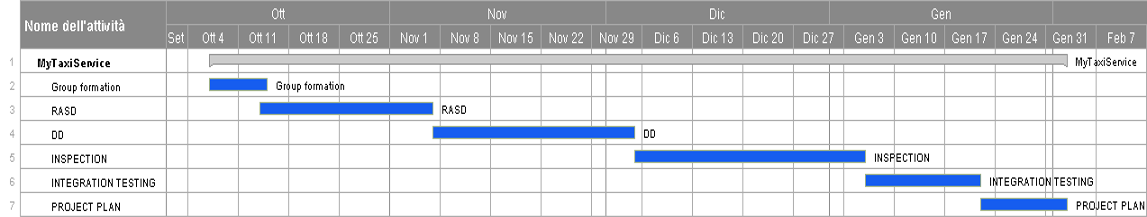
\includegraphics[scale=0.4]{chapters/SWE2-4.png}}

\caption{Gantt's diagram}
 \end{figure}
\end{center}


 \chapter*{Risk evaluation}
 \addcontentsline{toc}{chapter}{Risk evaluation}
 \setcounter{section}{0}
 \addtocounter{chapter}{1}
 \section {Risk evaluation and avoidance}

In this section we describe the risk identification: in Table 1 for each risk we assign a probability and the degree of seriousness, 
in Table 2 we define a plan to follow in case the risk occurs.\\
\newline
\begin{tabular}{  | l | l | l |}
    \hline
     Risk  & Probability  & Effects \\ \hline
    1.Key staff are ill at critical times in the project & Moderate & Serious  \\ \hline
    2.Changes to requirements that require major design rework & Moderate & Serious  \\ \hline
    3. Loss of data  & Low & Catastrophic \\ \hline
    4. Poor collaboration among team members & Moderate & Serious \\ \hline
\end{tabular}\\
\newline
\newline
\begin{tabular}{  | c |  p{14cm} |}
    \hline
    Risk  & Strategy \\ \hline
    1. & Each member is aware of the job done by other components so that he can review/finish the task if someone gets sick \\ \hline
    2. & Pay attention and if needed ask for clarification  \\ \hline
    3. & Keep all material synchronized with Github \\ \hline
    4. & Keep in good relationship and talk about the project issues \\ \hline
\end{tabular}

\end{document}    
